\chapter{Decorator}
\section{Intento}

Associare responsabilità aggiuntive a un oggetto in modo dinamico. I decorator forniscono un'alternativa flessibile all'ereditarietà


%---
\section{Prestruttura}

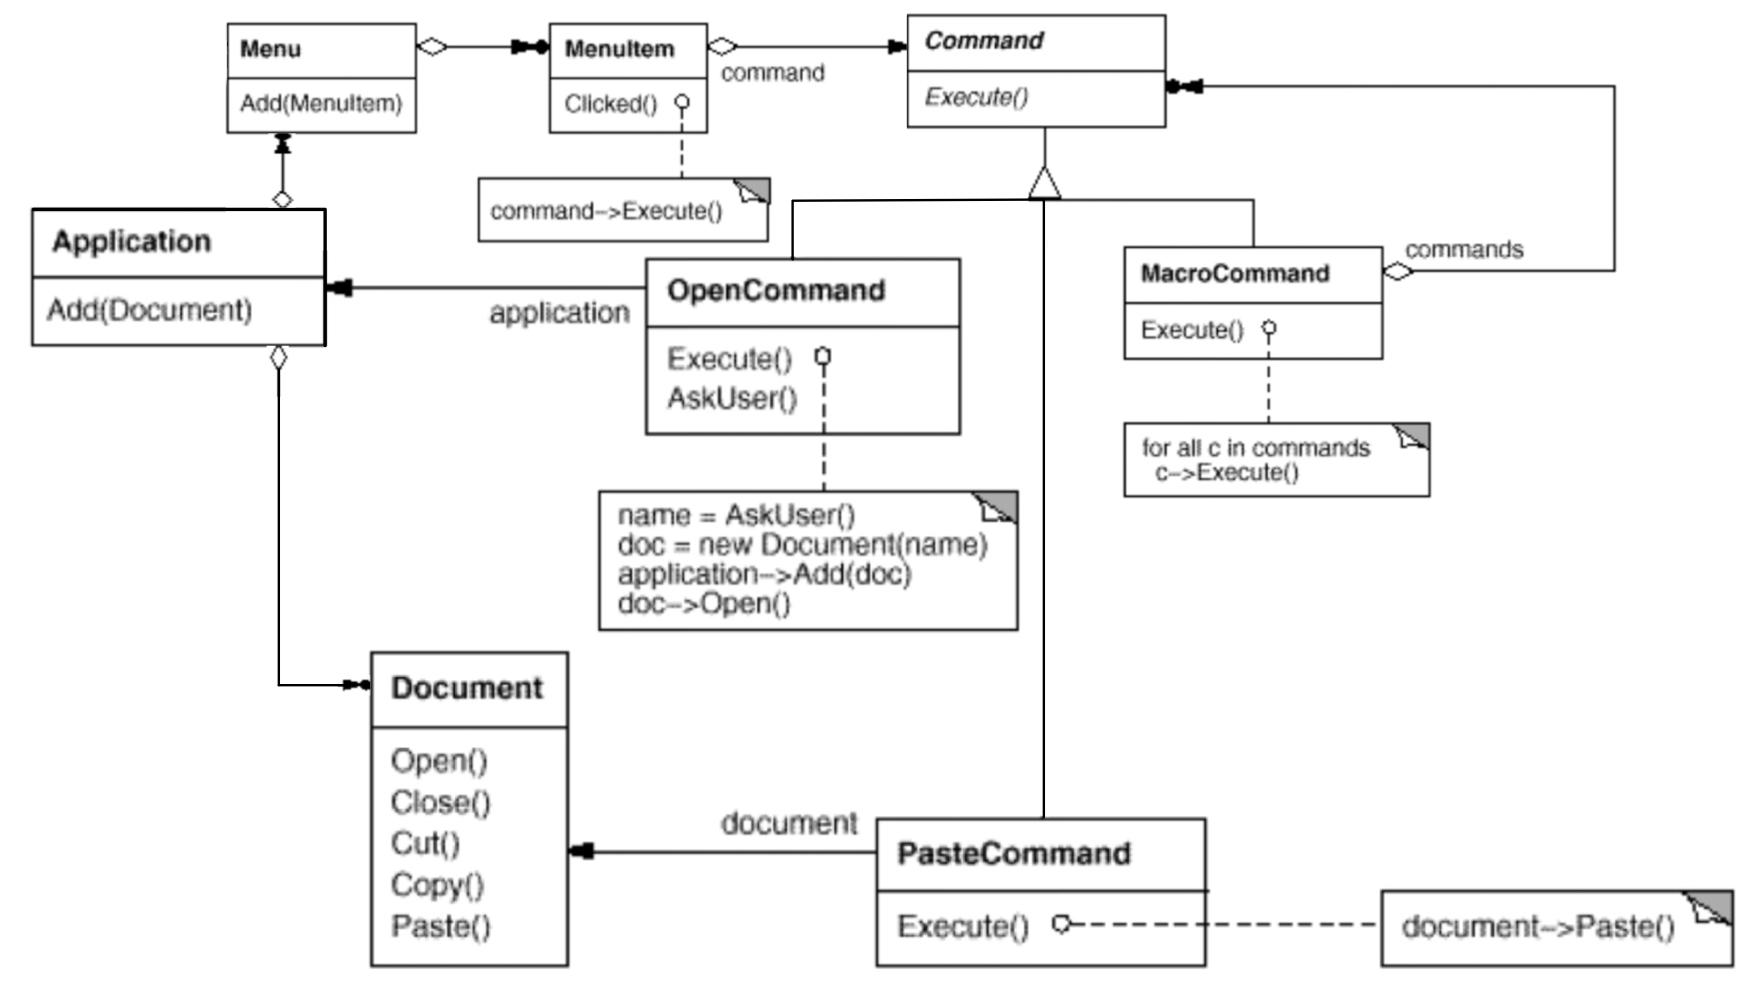
\includegraphics[width=\textwidth]{/Users/matt/Documents/LaTex/Design Pattern LaTex/Decorator/Prestructure1}


%---
\section{Struttura}

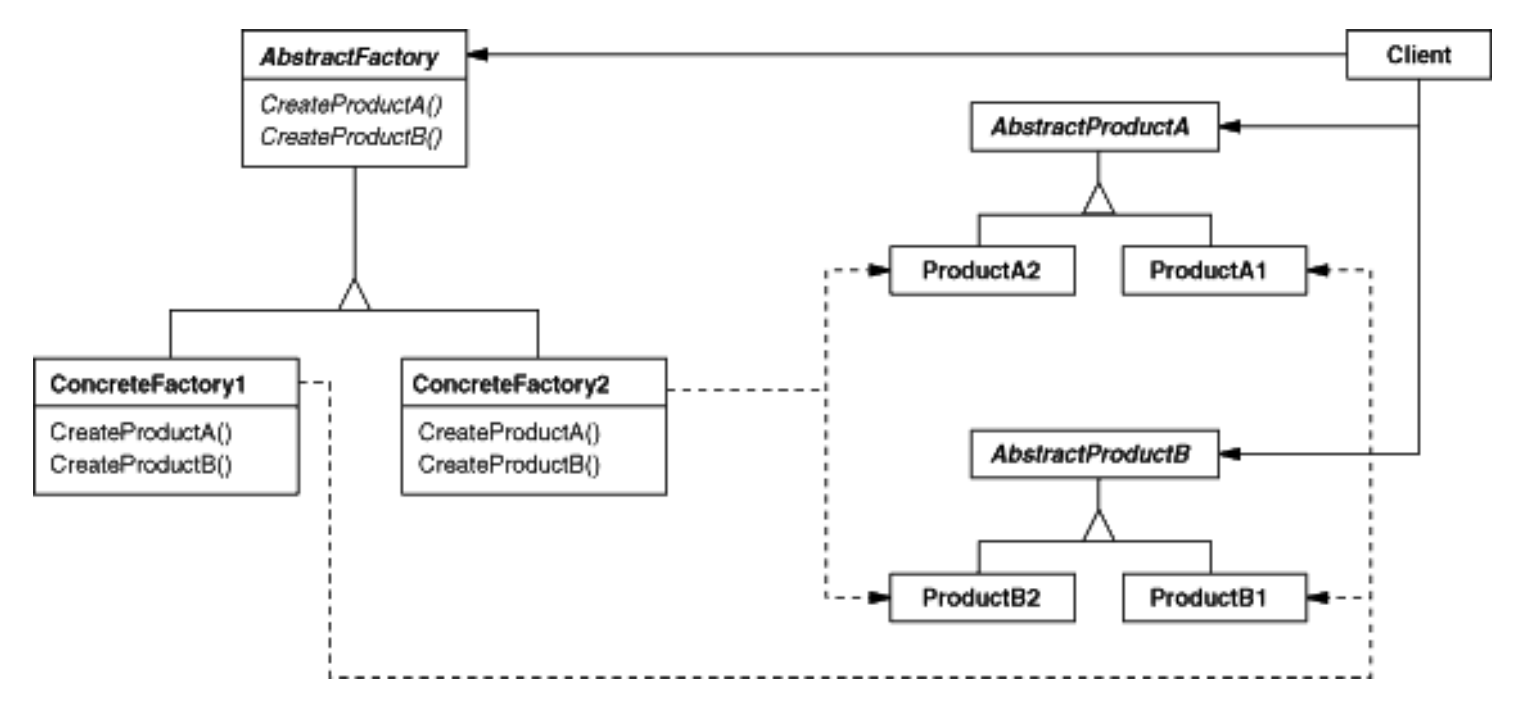
\includegraphics[width=\textwidth]{/Users/matt/Documents/LaTex/Design Pattern LaTex/Decorator/Structure1}


%---
\section{Implementazione}

\subsection{Omissione della classe di decoratore astratto.}
Non c'è bisogno di definire una classe di decoratore astratto quando è necessario aggiungere solo una responsabilità.Questo è spesso il caso quando hai a che fare con una gerarchia di classi esistente piuttosto che progettarne una nuova.

Puoi unire la responsabilità del decoratore per inoltrare le richieste al componente in ConcreteDecorator.

\subsection{Mantenere le classi dei componenti leggere.}
Per garantire un'interfaccia conforme, componenti e decoratori devono discendere da una classe Component comune.

È importante:

\begin{itemize}
    \item mantenere leggera questa classe comune, facendola concentrare sull'assomigliare ad un'interfaccia, non a memorizzare dati.

    \item la rappresentazione dei dati dovrebbe essere rinviata alle sottoclassi; altrimenti la complessità potrebbe rendere i decoratori troppo pesanti da usare in quantità.
\end{itemize}


%---
\section{Esempio Java}
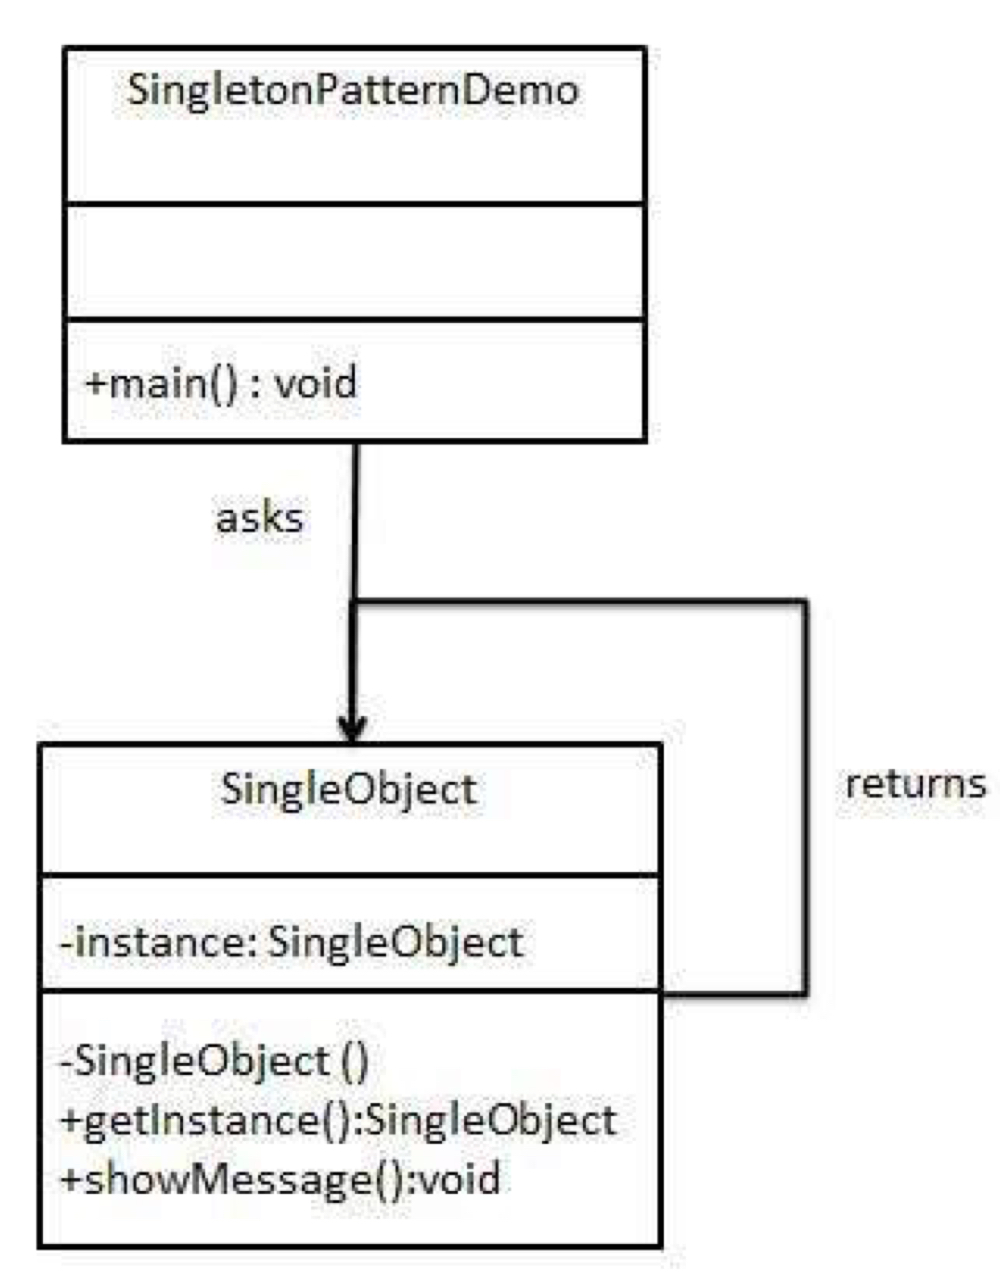
\includegraphics[width=\textwidth]{/Users/matt/Documents/LaTex/Design Pattern LaTex/Decorator/Example1}

\subsection{Shape.java}
\begin{lstlisting}[language=java]
    public interface Shape {
        void draw();
    }
\end{lstlisting}

\subsection{Circle.java}
\begin{lstlisting}[language=java]
    public class Circle implements Shape{

        @Override
        public void draw() {
            System.out.println("CERCHIO");
        }
        
    }
\end{lstlisting}

\subsection{Rectangle.java}
\begin{lstlisting}[language=java]
    public class Rectangle implements Shape {

        @Override
        public void draw() {
            System.out.println("RETTANGOLO");
        }
        
    }
\end{lstlisting}

\subsection{ShapeDecorator.java}
\begin{lstlisting}[language=java]
    public abstract class ShapeDecorator implements Shape{
        protected Shape decoratedShape;
    
        public ShapeDecorator(Shape decoratedShape) {
            this.decoratedShape = decoratedShape;
        }
    
        @Override
        public void draw() {
            decoratedShape.draw();
        }
    }
\end{lstlisting}

\subsection{RedShapeDecorator.java}
\begin{lstlisting}[language=java]
    public class RedShapeDecorator extends ShapeDecorator {

        public RedShapeDecorator(Shape decoratedShape) {
            super(decoratedShape);
        }
        
        @Override
        public void draw() {
            decoratedShape.draw();
            setRedBorder(decoratedShape);
        }
    
        private void setRedBorder(Shape decoratedShape) {
            System.out.println("BORDO ROSSO");
        }
    }
\end{lstlisting}

\subsection{main}
\begin{lstlisting}[language=java]
    public static void main(String[] args) {
        Shape circle = new Circle();
        
        Shape redCircle = new RedShapeDecorator(new Circle());
        Shape redRectangle = new RedShapeDecorator(new Rectangle());

        System.out.println("Cerchio normale:");
        circle.draw();

        System.out.println("Cerchio rosso:");
        redCircle.draw();

        System.out.println("Rettangolo rosso:");
        redRectangle.draw();
    }
\end{lstlisting}